\documentclass[10pt,a4paper]{article}

% Use this command to override the default ACM copyright statement (e.g. for preprints). 
% Consult the conference website for the camera-ready copyright statement.


%% EXAMPLE BEGIN -- HOW TO OVERRIDE THE DEFAULT COPYRIGHT STRIP -- (July 22, 2013 - Paul Baumann)
% \toappear{Permission to make digital or hard copies of all or part of this work for personal or classroom use is 	granted without fee provided that copies are not made or distributed for profit or commercial advantage and that copies bear this notice and the full citation on the first page. Copyrights for components of this work owned by others than ACM must be honored. Abstracting with credit is permitted. To copy otherwise, or republish, to post on servers or to redistribute to lists, requires prior specific permission and/or a fee. Request permissions from permissions@acm.org. \\
% {\emph{CHI'14}}, April 26--May 1, 2014, Toronto, Canada. \\
% Copyright \copyright~2014 ACM ISBN/14/04...\$15.00. \\
% DOI string from ACM form confirmation}
%% EXAMPLE END -- HOW TO OVERRIDE THE DEFAULT COPYRIGHT STRIP -- (July 22, 2013 - Paul Baumann)


% Arabic page numbers for submission. 
% Remove this line to eliminate page numbers for the camera ready copy
\pagenumbering{arabic}


% Load basic packages
\usepackage{balance}  % to better equalize the last page
\usepackage{graphics} % for EPS, load graphicx instead
\usepackage{times}    % comment if you want LaTeX's default font
%\usepackage{url}      % llt: nicely formatted URLs
\usepackage[utf8]{inputenc}
\usepackage{color}
%\usepackage{tabulary}
%\usepackage{amsmath}
\usepackage{array}

\usepackage[english]{babel}
%\usepackage[latin1]{inputenc} %Has danish letters
\usepackage[utf8]{inputenc}
\usepackage[T1]{fontenc}
%\usepackage{biblatex}
%\addbibresource{references}
\usepackage{graphicx}
\usepackage{wrapfig}
\graphicspath{{./pics/}}	%For images
\usepackage{appendix}
\usepackage{amsmath}
\usepackage{fixltx2e} %To use \textsubscript
%\usepackage[bookmarks]{hyperref}
\usepackage[nottoc]{tocbibind}
\usepackage{csquotes}
\usepackage{epsfig}
\usepackage{epstopdf}
\usepackage{framed, color}
\usepackage{xcolor,colortbl}
\usepackage{enumerate}
\usepackage{footnote}
\usepackage{siunitx} %SI units like micro and such
%\usepackage{geometry} %To put table in landscape
\usepackage{pdflscape} %To put table in landscape
\usepackage{pdfpages}
%\usepackage[style=verbose-trad2,backend=bibtex]{biblatex}
\usepackage[left=3.5cm, right=3.5cm,top=3cm,bottom=3cm,heightrounded]{geometry}
%\usepackage{todonotes}
\usepackage{hyperref}
\hypersetup{
	pdftitle={SIGCHI Conference Proceedings Format},
	pdfauthor={LaTeX},
	pdfkeywords={SIGCHI, proceedings, archival format},
	bookmarksnumbered,
	pdfstartview={FitH},
	colorlinks,
	citecolor=black,
	filecolor=black,
	linkcolor=black,
	urlcolor=black,
	breaklinks=true,
}
%\usepackage[hyphens]{url}

%\usepackage{float}


\definecolor{Orange}{rgb}{1,0.5,0}
%\newcommand{\todo}[1]{\textsf{\textbf{\textcolor{Orange}{#1}}}}

\title{Towards a generic dispenser module for laboratory platforms}
\author{
	Lars Yndal Sørensen, MSc. Stud., lynd@itu.dk\\
	IT University of Copenhagen\\
	Rued Langgaards Vej 7, 2300 Cph S\\
}
\date{May 2016}

%\toappear{Paper submitted for evaluation in an elective project, spring 2016. The IT University of Copenhagen. Copyright remains with the author.}


% End of preamble. Here it comes the document.
\begin{document}

	\begin{titlepage}
		\maketitle
		\thispagestyle{empty}
	\end{titlepage}

	\tableofcontents
	\newpage
	
	
	
	\section{Abstract}
		A lot of public and private institutions are using laboratory platforms and liquid-handling robots today, when i.e. researching or testing human health related issues. These platform are mainly developed by the industry, because they were needed and not in the "normal" way of research, where ideas are combined to see if borders of what is possible can be moved.
		
		This results in, that only minor public research has been done in this field, which has left the industrial platforms to be designed in ways that aims at only addressing very few processes for each platform - each process may be used to different experiments, though, if different chemicals are used. Each platform often also come as \textit{one} unit and is hardly modular, which limits start-up companies and institutions with little finances to acquire such products.
		
		To change this rigid way of designing laboratory platforms, this project will design the first step towards a more modular approach of the laboratory platforms: A dispenser module. The module will be designed to handle both Petri dishes and multiplates, while addressing issues like, i.e. responsiveness and usability.
		
	\newpage
	
	
	
	
	
	
	
	
	
	
	
	
	
%	SciRobotics Ltd.
%		http://www.scirobotics.com/solutions/petrilab
%	Tecan (can swap end manipulator tools)
%		http://lifesciences.tecan.com/products/liquid_handling_and_robotics
%	Retisoft Inc
%		http://www.retisoft.ca/hardware/flex.php
%		http://www.retisoft.ca/solutions/dna-snp.php
%	Beckman Coulter
%		http://www.beckman.com/liquid-handling-and-robotics
%	Labcyte
%		http://www.labcyte.com/products/automation/labcyte-automation
%	TTP Labtech
%		http://ttplabtech.com/liquid-handling/
%	JEL Corporation
%		http://www.jel-robot.com/products/PETRI.html
%	Hudson Robotics, Inc.
%		http://hudsonrobotics.com/products/microplate-handling/
%	Agilent Technolgies
%		http://www.agilent.com/en-us/products/automation-solutions/microplate-management-robotics/direct-drive-robot
%		http://www.agilent.com/en-us/products/automation-solutions/microplate-management-robotics/benchbot-robot
%	Festo
%		https://www.festo.com/cat/da_dk/products
%	Neotec Bio
%		http://neotec.co.il/automation/
%		http://neotec.co.il/robotics/
		

	\section{Introduction}
	
	A lot of public and private institutions are working with laboratory platforms to perform experiments in Petri dishes or multiwell plates. These experiments are often related to human health or other biological research. As each of these types of experiments often are best fitted to be done in \textit{either} the multiwell plates or the Petri dishes, the laboratory platforms are often designed to work with one \textit{or} the other.
	
	In rare cases\cite{tecan_webpage} the end manipulator of the platform is able to actually change head tools during an experiment and thereby serve multiple functions - including handling both  plates and Petri dishes.
	
	Even if the laboratory platforms are build from different small stations that can be seen as modules, it seems like this approach hasn't really got to the manipulating of the plates yet. 
	As the old saying of \textit{"the chain is not stronger than the weakest link"}, one could easily argue that, \textit{almost} having a system that supports multiple types of plates is the same as \textit{not} having a system that supports multiple types of plates!\\
	
	Public and private institutions that use platforms may, for several reasons, not be interested in platforms that are limited to a small amount of types of experiments. These reasons may be related to financial circumstances, or because they just need to perform a limited series of experiments, before turning to a completely different type of experiments. This rules out the use of available laboratory platforms, in which case, some institutions are creating their own platforms to address their specific needs.
	
	To address the high prices of these laboratory platforms, and thereby make such available to the majority, this report will take the first step towards this and design a low-cost dispensing module. The module will be able to handle several types of experiment dishes, while also supporting removal of used plates.\\
	
	The rest of this report will focus on the mechanical design of the module, describing everything from the initial design goals, through each design iteration and the results.
	
	Due severe problems from the hardware supplier, this entire project has suffered a large set-back in terms of testing the mechanical design and a conclusive integrated experiment. Even though a large piece of the firmware for the module has been written, the lack of materials made is impossible to test and adjust the code. Therefore the mechanical design is only tested in non-trivial situations, by writing small code pieces, simulating the actual behaviour. More trivial, but time-consuming, firmware actions, i.e. vertical and horizontal movements are instead tested by hand.
		
	\newpage
	
	\section{Design goals}
	In order to increase the design and clarify the important functionalities needed, a series of user scenarios will be described. The concrete design goals will be extracted from these and kept in mind through-out the design process, and be used to evaluate the proposed system at the end.
	
	\subsection{User scenarios}
	5 scenarios, describing the users's situations.
	
	
	\begin{enumerate}
		\item \textbf{Adding dispenser module to a platform}\\
		If a user has a laboratory platform and wants to increase the automation, she can easily integrate the dispenser module with only minor modifications.
		
		\item \textbf{Different types of plates}\\
		To broaden the possibilities with the dispenser module, it must be able to handle different types of dishes/plates. The user shall not need to define which that are inserted into the module, as the module must be able to detect this automatically.
		
		\item \textbf{Adding/removing dish stacks}\\
		While the dispenser is running, it must be straight forward to add and remove containers with dishes/plates. The user must not be concerned about the state of the dispenser, as the dispenser must adapt to the user's actions in runtime.
		
		\item \textbf{Breakage}\\
		The module may at some point be worn down or parts may break. When this happens, the parts must be easy and low-lost to replace.
		
		\item \textbf{Concurrent }\\
		The device controlling the dispenser module, will get requested data from the dispenser module, no-matter what state the dispenser module is in. The module should be dependent on the controlling device, not the other way around.
		
		
	\end{enumerate}
	
	\subsection{Goals}\label{subsec_Goals}
	In the described user scenarios, there are several situations that must be addressed. These are listed below:
	
	\begin{itemize}
		\item \textbf{Modularity} Able to attach/remove the dispenser module without any hassle.
		\item \textbf{Versatility} Address different sizes of Petri dishes/multiplateswells.
		\item \textbf{Usability} Easy to add/remove stacks of Petri dishes/multiplates during runtime.
		\item \textbf{Flexibility} Can be attached to the majority of current laboratory platform modules.
		\item \textbf{Increased feedback} Detects the platform layers automatically.
		\item \textbf{Repairability} Easy to create spare parts - and low cost.
		\item \textbf{Responsive Control} Attached controller must be able to send commands and get responses from module regardless of any ongoing motions, et.c.
	\end{itemize}
	\newpage
	
	\section{Mechanical design}
	
	As the module shall be available to the largest amount of people, the design is based on open-source\footnote{The open-source parts are available around the world, but technical details can be found at \url{www.openbuildspartstore.com} and \url{www.pjrc.com/teensy}.} and non-specialized parts. The choice of this is to allow the user to either produce them by himself or acquire them at a low cost, and thereby increase the availability of this dispenser module to the world. 
	
	This section will continue in an iterative way, starting by describing the initial thoughts toward the first prototype and the design choices, emphasizing key features like the gripper functionality, layer detection and the dish containers. At each iteration, the prototype will be evaluated at these features plus on a general level.
	
	All of the mechanical design is created using SolidWorks 2015\cite{solidworks_webpage} and can be found at GitHub\cite{github_dispenserProject} along with the developed software, etc.
			
	\begin{wrapfigure}{r}{0cm}
		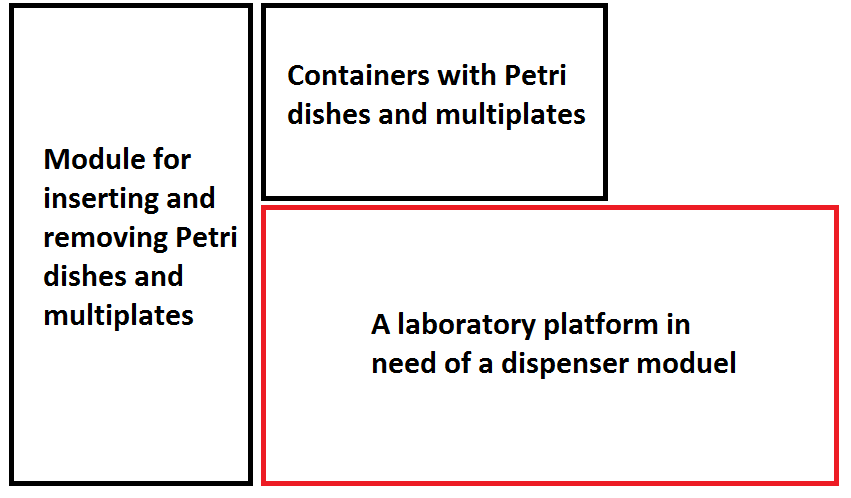
\includegraphics[width=6cm]{images/platformOverview.png}
		\caption{Overview of the dispenser module ({\color{black}\textbf{black}} squares) next to a laboratory platform ({\color{red}\textbf{red}} square). Notice how the area above platform serves as storage for both clean and used dishes/multiplates, while the left area is for the insertion/removal mechanism.}
		\label{fig::platformOverview}
	\end{wrapfigure}
		
	\subsection{Initial design}\label{subsec:intialDesign}
		
	Since the dispenser module must fit most laboratory platforms, it must have a generic overall set up: Most currently available platforms seem to have divided their space into 3 main areas: 1) a primary area of a surface with a bit of free space above for placing, manipulating and moving the dishes and multiplates, 2) below the primary area there may be some devices for analysing or growing the sample, and 3) an area above the primary area where mechanical tools for performing the placing, manipulating and moving are mounted and positioned.
	
	\begin{wrapfigure}{r}{0cm}
		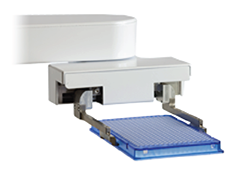
\includegraphics[width=6cm]{images/retisoftManipulator.png}
		\caption{Example of an end manipulator with two "fingers". This one is designed by Retisoft\cite{retisoftFlex_webpage}.}
		\label{fig::retisoftManipulator}
	\end{wrapfigure}
	
	As with much other equipment the design reminds of a cubic box, where the processes are handled within. By placing the dispenser module next to platform, it will be able to interact with the platform and retract it tools, when they are not needed, to prevent collisions with the platform's tools. On top of the platform, the containers for Petri dishes/multiplates will be placed, to save space horizontally, which is were most people first seem to run out of space compared vertically. To see an overview of the dispenser module next to a laboratory platform, please see figure \ref{fig::platformOverview}.
	
		
	\subsubsection{Gripping functionality}	
	The gripping functionality of the module is one of the primary functions and a severe amount of prior research has gone into this. Unfortunately, there is not much public available research in this area, for which reason, inspirational thoughts have come from industrial developed and proved designs.
	
	Many of the robots are designed to grip a Petri dish, multiplates or test tubes by simply squeezing two (often metal) arms from each side of the target.
	%dishes: jel and scirobotics and tecan
	Those handling multiplates\cite{agilentTechnologies-benchBotRobot_webpage} \cite{agilentTechnologies-directDriveRobot_webpage} \cite{festo_webpage}  \cite{hudsonRobotics_webpage} \cite{labcyte_webpage} \cite{neotecBio-automation_webpage} \cite{neotecBio-robotics_webpage} \cite{retisoftDnaSnp_webpage} \cite{retisoftFlex_webpage} \cite{tecan_webpage} \cite{ttpLabtech_webpage} often have two "fingers" with small shapes at the end (see figure \ref{fig::retisoftManipulator}). These shapes allow the manipulator to get a hold of, i.e. the bottom of the plate without touching a potential lid. Other designs have a sort of palette that supports the lifting with a good hold from the bottom instead of relying on a friction-based grip, that requires additional force added to the sides of the plate. 
	
	\begin{wrapfigure}{l}{0cm}
		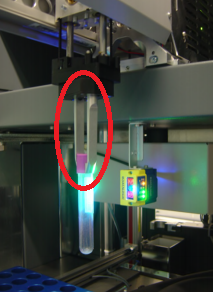
\includegraphics[width=4cm]{images/tecanTestTube.png}
		\caption{End manipulator ({\color{red}\textbf{red}} circle) from Tecan\cite{tecan_webpage} holding a test tube.}
		\label{fig:tecanTestTube}
	\end{wrapfigure}
		
	Those\cite{jelCorporation_webpage}\cite{scirobotics_webpage}\cite{tecan_webpage} handling Petri dishes are very similar to those for multiplates, but the "edges" at the end of the fingers are a bit concave to have more than two points where the dish is gripped\footnote{If the grip of a Petri dish only has two points, there is a high risk of the dish tipping or even get dropped during the lift or repositioning.}. Some designs have addressed the two-point-issue by adding two vertical plastic cylinders at the bottom of each arm to center the dish while performing the squeeze mechanism. The outer part of the arm, are in some of these cases a bit flexible to help the centering even better, but mainly the end of the arms were fixed.
	
	The manipulators for test tubes remind of those for Petri dishes, but the form factor is smaller and the arms are all vertically. The end or the arms were also shaped to fit the used test tubes - when closed, the arms would almost be in contact with the test tube all the way around (see figure \ref{fig:tecanTestTube}).
	

	
	One of the end manipulators, which actually \textit{was} from the research world, was PetriJet\cite{petrijet_ding2015jala}. This machine is capable of moving a Petri dish from one stack, to a camera for analysis and then to another stack. The PetriJet uses a suction cup for moving the dishes, which implies that Petri dishes with lockable lids were used. The same goes for some of the industrial developed manipulators, which are used for test tubes, as these were lifted by a suction cup in touch of the rubbery center of the test tube's cap. The proposed system should be able to not only handle dishes and plates with lids, but also without lids - therefore a suction cup can't be used.
	
	Among the found laboratory platforms, only a single had the capability to change end manipulator end at run-time\cite{tecan_webpage}. The Tecan end manipulator was used to not only handle well plates, but also test tubes at the same time, which required the dynamically change of tool for the end manipulator.\\
	
		
	
	%A few of the industrial solutions had designed a small squared plate, where a Petri dish was placed. This prevented the end manipulator from actually grip the dish as a simple fork-inspired design could slide in between two plates, separated by a Petri dish, and lift up the top plate and a the Petri dish placed on top of it. \todo{Picture?}
	
	%Such an approach opens op the opportunity to mark each squared plate with a barcode or similar. A picture taken from an experiment could then include this barcode as reference.
	
	%To save material and avoid stacks of Petri dishes, that will slide out of position, the squared plate is rejected for now, but noted as a potential solution to forthcoming issues.
		
	\begin{wrapfigure}{r}{0cm}
		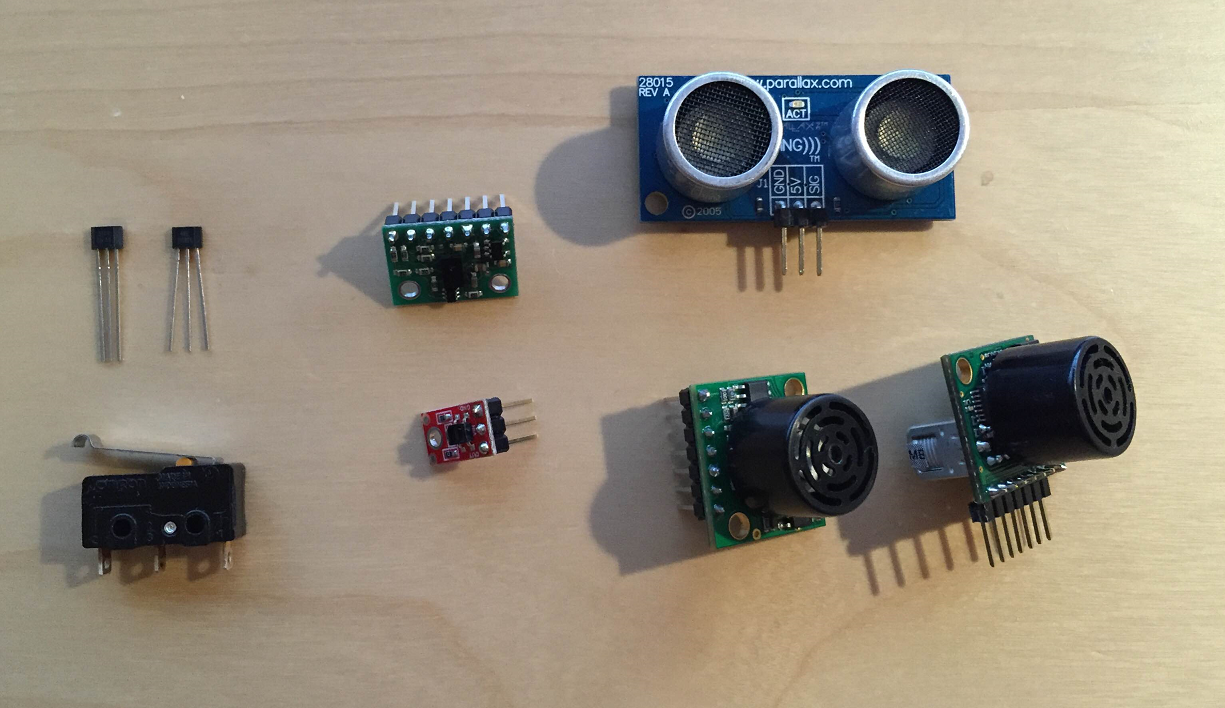
\includegraphics[width=6cm]{images/sensors.png}
		\caption{The tested sensors: 3 ultrasound (right), 2 hall effect (upper left), 1 level switch (lower left) and 2 IR (center)}
		\label{fig::sensors}
	\end{wrapfigure}
	
	Based on the aforementioned background research, the initial design of the gripper will be based on two arms, that respectively will have one and two points of contact with the dish/plate. The end of the arms will be fixed to ensure that, i.e. a misaligned well plate will be correct aligned while the grip is achieved. The reason for having a total of three and not four points of contact is to minimize complexity. Some high-friction material will be added at the contact points to give a better grip.
	
	During the initial design several sensors will be mounted at the end of the arms. These sensors are of different types, but addresses some of the same issues. Please see \nameref{subsub:Initial_LayerDetection} for details about this.


	\subsubsection{Layer detection}\label{subsub:Initial_LayerDetection}
	Layers, in the proposed system, is to be understood as, i.e. the platform where all experiments are conducted or the layers of tools above/below the platform layer. A layer is static in terms of height but tools and other equipment in the layer can freely be moved around.
	
	
	Detecting the layers in the module, is to increase the user experience, when determine which layer to insert/remove dishes and plates to/from, as this otherwise could be done manually. In this way, the proposed module can also be used together with laboratory platforms, where such layers can be adjusted dynamically and complement this by telling the new heights - if the platform itself is not capable of this already.
	
	Amongst the found research projects and industrial robots, none had addressed this issue about detecting layers of external equipment before. Thoughts go towards, that often the layers are permanently mounted or simply not existing, for which reason it hasn't been seen as a problem. With the constant development of this technology and only more dynamic solutions will be designed, this will still be considered as an important design feature - in this way, the proposed module can also be matched with future laboratory platforms.
		
	As the detection of layers are to be implemented, it might as well be used to detect heights of dishes/plates in a container (see \nameref{subsubsec:Initial_DishContainers}). To detect these heights, several solutions will be implemented in the gripper for the initial design. This is to compress the overall process and test multiple solutions at once. The sensors are all standard sensors and of the following types:
	
	

		
	\begin{itemize}
		\item \textbf{Ultrasound sensors}\footnote{Two of the ultrasound sensors tested ar efrom MaxBotix and has part number MB1000 and MB1202. The third is a Ping))) from Parallax.} Ideal for this scenario as physical contact is avoided, the cost is low and precision is high. Three ultrasound (US) are tested, which both has a narrow beam to prevent false distances.
		\item \textbf{IR sensors} The IR sensors will also avoid physical contact, but distances are much closer compared to an US sensor. One of the IR sensors\footnote{The low-cost IR sensor is from Pololu with item number 2458.} is very standard and low-cost, while the other\footnote{The IR sensor with the high-end, build-in filter is also from Pololu and has item number 2489.} has a high-end, build-in noise filter to external light.
		\item \textbf{Level switch} Widely used standard level switch also known as endstop. Requires physical contact, which can be an issue when detecting height of clean dish/plate stacks, but very low cost and reliable.
		\item \textbf{Hall effect sensors}\footnote{The parts numbers for the hall effect sensors tested are: 3144 OH14 (linear) and 49E 11082N (switch).} Requires a magnetic element as the target to be detected, which will be an issue when detecting the height of dishes/plates, but low cost and commonly used with no need for physical contact. Two\footnote{The third type of hall effect sensors is a Latching Hall Effect sensor, which holds the logical value until it is unlatched by a reversed polarity. This type is left out as it would require the magnets to dynamically be turned around.} types of hall effect sensors are tested: Switch and linear ratiometric.	
	\end{itemize}
	
		
	\subsubsection{Dish containers}\label{subsubsec:Initial_DishContainers}
	
	The dish containers, that are placed on top of the platform, are those that hold the clean/unclean dishes. It is unrealistic to create \textit{one} container, that will fit all possible variations of Petri dishes and multiplates. Therefore two designs will be create: One for holding the multiplates, which have the same size independently of how many wells that actually are, and one design for Petri dishes with a diameter of 93mm. Both containers can then be resized to fit other sizes of the dishes/plates.
	
	
	
	The way that the module will detect a container being added/removed and what type of dishes is done by placed a small resistor in the bottom of the container - there is actually room for a PCB of 76-81x60 mm, depending on the container, which is more than enough for a small resistor and some pressure-released contacts. \textit{If} it is not feasible to detect the height of the dishes by a gripper mounted device, a distance sensor can be located in the top dish container and a micro controller, if needed, can be placed in the bottom to report the amount of dishes to the dispenser module.
	\\
	
	
	The designs of the two containers are rather similar, as it enclose the dishes/multiplates by sheets of 3mm POM and has a skeleton of 20x20 mm alu profiles (see figure \ref{fig:initialContainer} for the dish container). At first it was considered to use rods for supporting the dishes and plates, but designing a stable structure for this, turned out to be more complex than first thought. Therefore the design continued by using the POM sheets.
	
	
	For both designs, the front sheet has been tilted a few degrees to align the dish/plate as it is being placed into the container, in case it is misaligned. The container for the Petri dishes has a cut in each side, which is a few millimetres narrower in the bottom compared to the top. This is to align the dish in the other direction while it is being lowered into place.
	
	\begin{wrapfigure}{r}{0cm}
		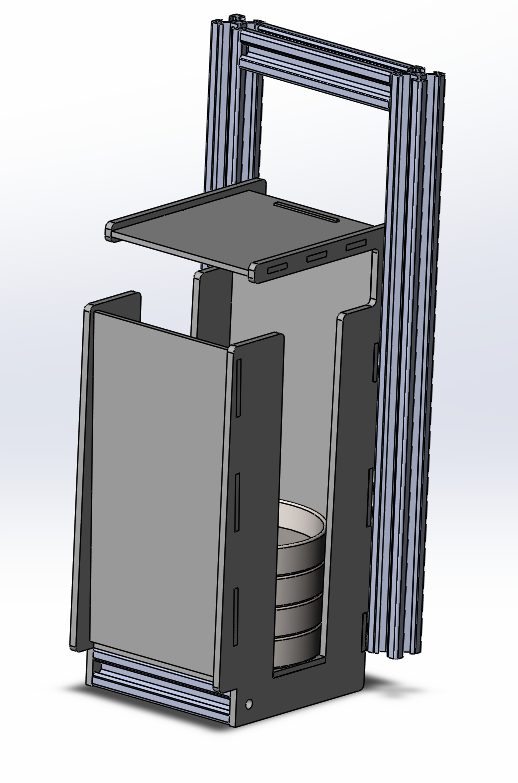
\includegraphics[width=6cm]{images/initialContainer.png}
		\caption{The initial design of the dish container, which is very similar to the plate container.}
		\label{fig:initialContainer}
	\end{wrapfigure}
	
	The front of container for the multiplates is much more open, and consists of only a single vertical bar supporting the plates. As the two farthest away corners are holding the multiplates into position together with the front, it should be plenty for keeping the multiplates in a correct position.
	
	The container for the multiplates is designed without a top, opposite the container for the dishes. This is to test with and without the tops during this initial run.
		
	
	\subsubsection{Misc. design decisions}
	
	\begin{wrapfigure}{r}{0cm}
		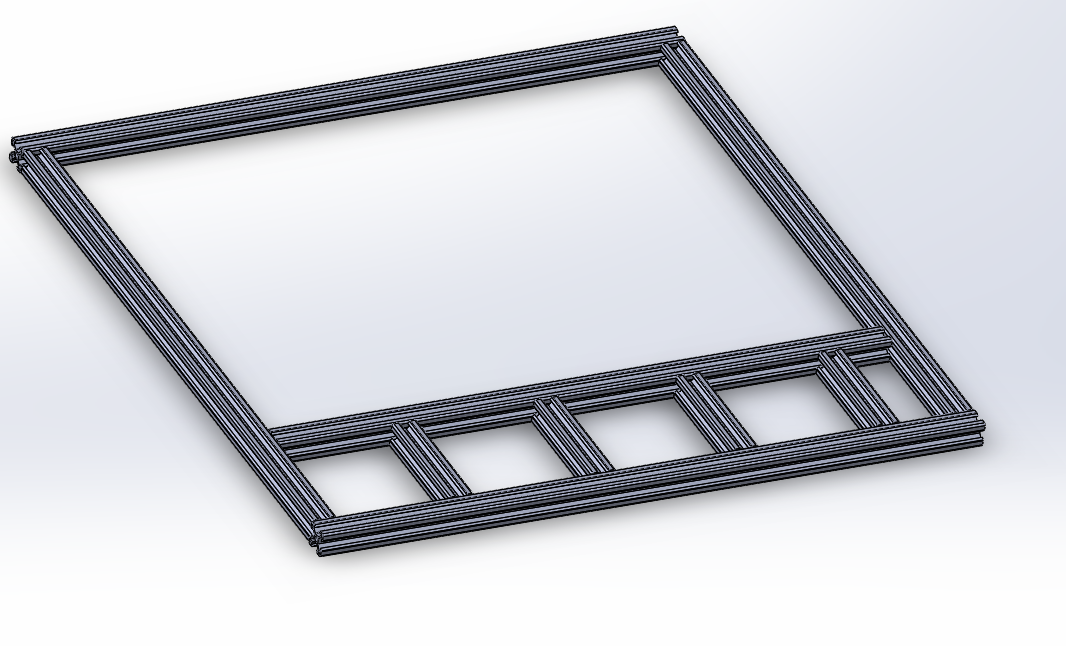
\includegraphics[width=6cm]{images/containerPlatform.png}
		\caption{The container platform, which has been designed to separate each dish/plate from each other, by an 20x20 mm alu profile (lower area of the platform).}
		\label{fig:containerPlatform}
	\end{wrapfigure}
	To make sure that the dish containers wouldn't be misaligned or placed in wrong positions, compared to where the dispenser module believe the dish containers can be placed, there is first created a basic platform for the dish containers. This platform is going to be placed on top of the laboratory platform and will separate each dish container from the others by an alu profile - just like an alu profile will force the user to put the dish container in the very end of where the dispenser module is located (see figure \ref{fig:containerPlatform}).
	
	
	\subsection{1st iteration}
	The initial design was rather successful, but left room for some improvements. During the use of the materials, it was experienced that, i.e. the POM sheets could be used to hold metric screws in place by making the hole 1.2mm smaller and eventually creating a threads with the appropriate tools. This would save the hassle of holding a nut and a device, to be mounted, in place while turning the screw - not to mention actual saving the screw itself.
	
	The idea of placing the dish containers on top of the laboratory platform worked well, as no part of the platform could interfere with the dish containers.
	
		\subsubsection{Gripping functionality}
			\begin{wrapfigure}{r}{0cm}
				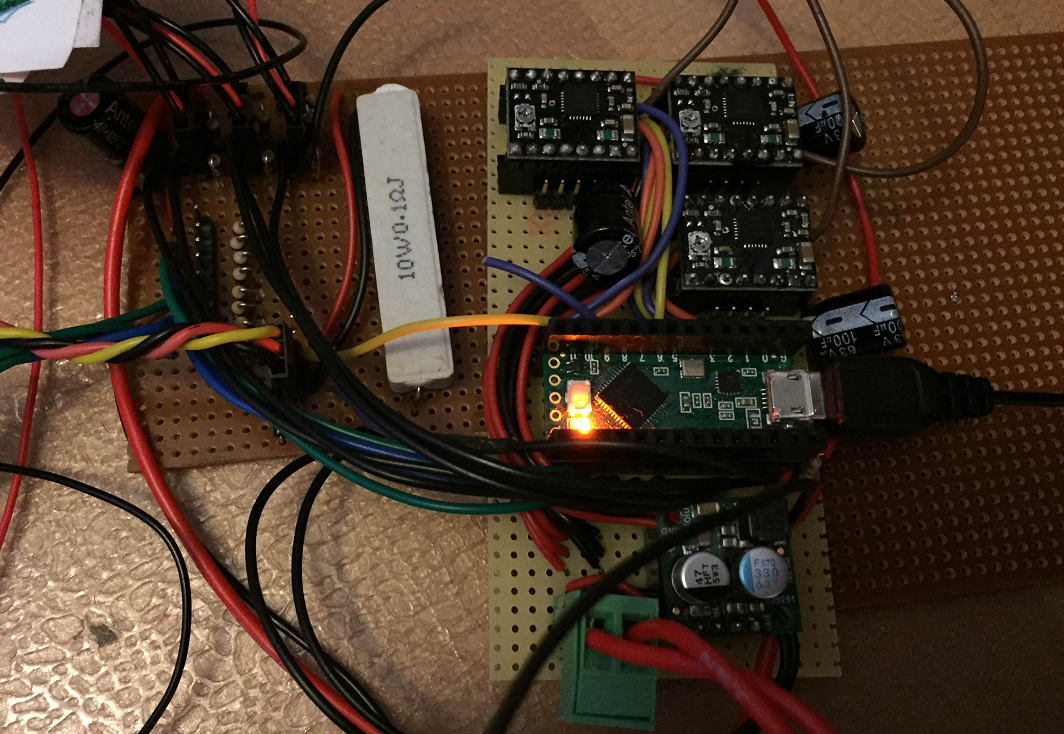
\includegraphics[width=6cm]{images/pcb.png}
				\caption{Image of the simple PCB for controlling the dispenser module.}
				\label{fig:pcb}
			\end{wrapfigure}
			
			The gripper worked rather well, even though the long arms would bend down ~3 mm when lifting a glass dish half filled with water. The Igus DryLin\textregistered N rails\footnote{\url{http://www.igus.com/wpck/3587/drylin_n}} gave a more firm motion than one could have thought: Even though they aren't designed to stabilize in the perpendicular direction, they did so very well. Thoughts about adding a third rail in the very front of the gripper to support the longest of the two arms, are rejected as the gain seems too small and it could misalign the longest arm compared to the shorter one when weight is added. This is unless a fourth rail is added farthest away and the shortest arm is extended to reach this rail (see figure \ref{fig:fourRails}).
		
			The servo controlling the two arms did a good job during the tests, even though the screw holes in the POM wasn't completely aligned with those in the servo. To measure the amount of force the arms would press against the dishes and multiplates, a simple electrical circuit was created (see figure \ref{fig:pcb}) allowing the micro controller to stop when enough force was added. It turned out that because the servo wasn't very strong, this wasn't necessary and that the servo would apply a reasonable amount of force when set to move the arms nearest to each other. Considering that the pressure was only going to be applied during movements of dishes and plates to/from the containers on the top and the laboratory platform, which is estimated to take less than 10 seconds, the risk of frying the servo wasn't seen as a problem.\\
							
			\begin{wrapfigure}{l}{0cm}
				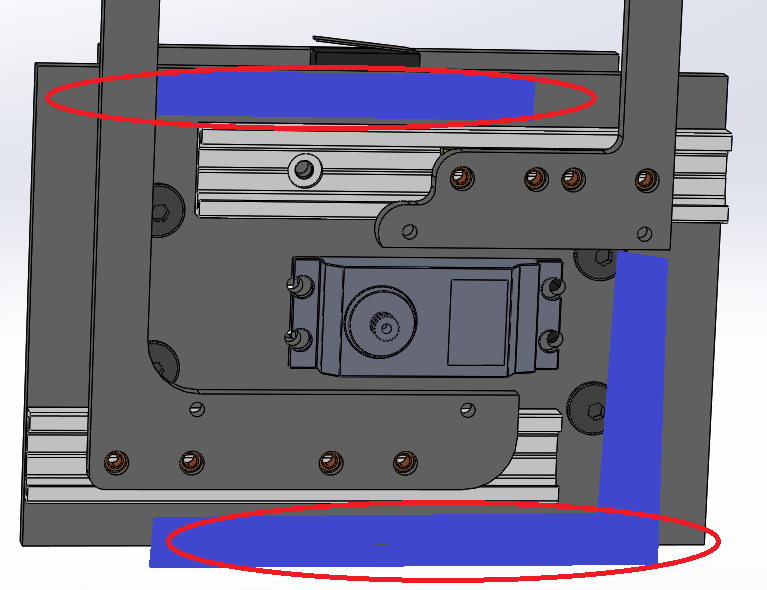
\includegraphics[width=6cm]{images/fourRails.png}
				\caption{Image of gripper from the bottom. The {\color{red}\textbf{red}} circles indicates, where extra rails can be added to increase stability to each of the two arms, if they were extended to also include the {\color{blue}\textbf{blue}} area.}
				\label{fig:fourRails}
			\end{wrapfigure}
			
			The motion of the entire gripper worked very well: It is smooth but firm at the same time. This was mainly achieved by using ball bearing in all the wheels and eccentric spaces in one of the sides. It was a bit difficult to adjust the eccentric spacers because of the compressed design.
			
			The positioning of the endstops worked good, as it was impossible to create a collision between the gripper and rest of the module unless an endstop was triggered first.
			
			The plastic rack and pinion used for transferring force from the servo to the arms was problematic as the initial design was with 3mm POM for the arms. The dimensions of the servo, the rails and the arms gave a misalignment between the rack and the pinion. But by using 6mm POM instead of the 3mm, the rack and the pinion is only off by 0.5mm and touching at 2.7mm.
			
			\begin{wrapfigure}{r}{0cm}
				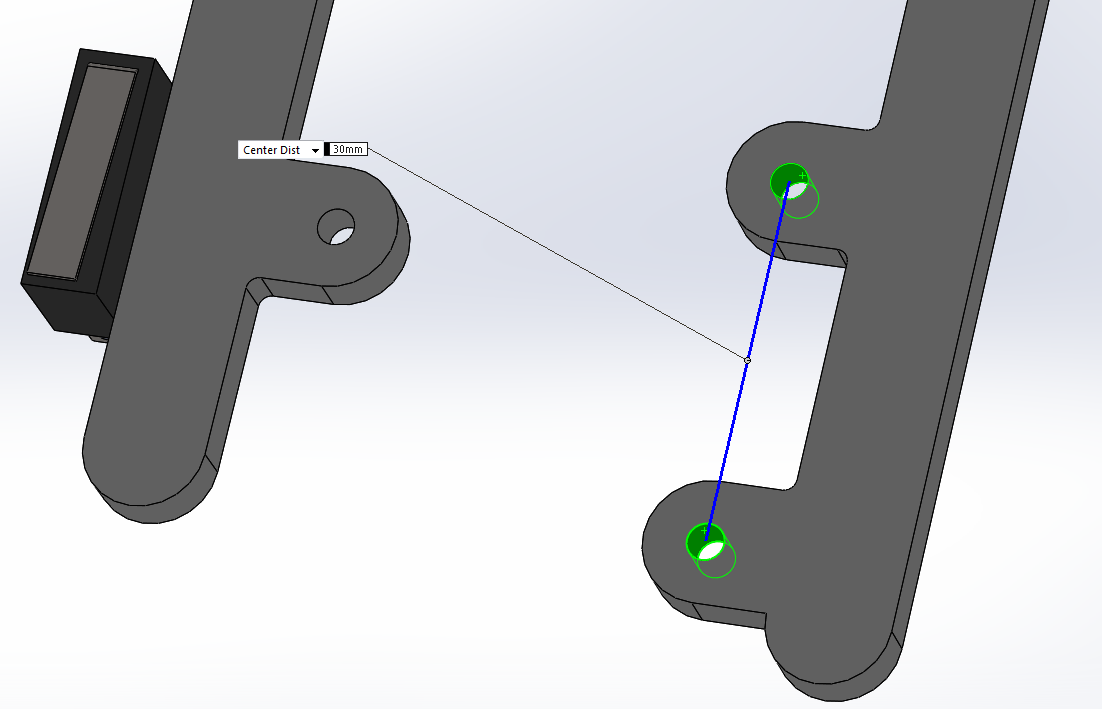
\includegraphics[width=6cm]{images/fingersFartherAway.png}
				\caption{Fingers with the new distance of 30mm to have a more stable grip during movement of dishes and plates.}
				\label{fig::fingersFartherAway}
			\end{wrapfigure}
			
			In order to compress the design even further and allow the gripper to handle objects that are even smaller, the sledges inside the rails have been moved closer to each other. The gripper can now manipulate a squared object, that has a width of only 32mm. In order to get a better grip, the two fingers on the one arm have been moved farther away from each other. This will give a larger holding area and increase the stability during the movement of dishes and plates (see figure \ref{fig::fingersFartherAway}). 
			
			Another thing that was changed in this iteration to compress the overall size of the gripper, is the two 40x20 alu profiles guiding the gripper: By changing them to 20x20 and using 4 corner brackets, a total of 25mm was saved. Unfortunately, the extra space for the corner brackets prevented a saving of all 40mm.
			
			A last thing that is changed in this iteration is the points of contact for the gripper: Instead of using 3mm with a rubber tube (for friction), they are turned upside down and their heads are used as points of contact. Hopefully this allow for lifting an entire Petri dish in \textit{one} turn instead of first moving the lid and \textit{then} the bottom.
				
		
				
		\subsubsection{Layer detection}\label{subsub::1iterationLayerDetection}
		The iteration of the layer detection focused on the different sensors (see figure \ref{fig::sensors}) and how their performed:
		
		
		
		\begin{itemize}
			\item \textbf{Ultrasound sensors} The three ultrasound devices were all able to detect the distance rather precise. But, unfortunately, 2 of them (those from MaxBotix) needed at least ~20 cm between the US sensor and the object to be detected. The one from Parallax, which has both an emitter and a receiver, only needed 3 cm - in some cases it could detect as low as 2 cm, but not reliably. All of them were able to detect both plastic and glass Petri dishes as well as the plastic multiplates. The size of the Parallax sensor is too big to be mounted at the tip of the gripper and thereby use it for not only detecting the amount of dishes/plates in a container, but also the layer heights. Placed in the top of a container, the sensor could be well suited to estimate amounts of dishes/plates that are in a container based on the heights of the stack.
			
			Another fact that speaks against the use of US sensors for layer detection is that they might get false positives and provide the distance to not the next layer but maybe a reflection of the dispenser module itself. 		
			
			\item \textbf{IR sensors} The very low-cost IR sensor was very sensitive to external light and can \textit{not} be used as this would require a completely static environment, which is impossible for the mere reasons that the module will have to move the sensor in order to detect the different layers.
			
			The VL6180X was still a bit sensitive to external light, but because of the build-in filter, the distance was mainly affected under extreme light conditions\footnote{The extreme light conditions in relation to the VL6180X was 50w halogen lamp pointed directly into the sensor.}. On the other hand, the reflection of different materials returned different distances: Tested in the dish container with a POM bottom, the lowest reliable distance was 21 mm, while the lowest reliable distance on a wooden desktop was 8 mm. The reason for this might be aforementioned built-in filter and the length of the wave lengths reflected by the surfaces.
			
			\item \textbf{Level switch} The level switch mounted the side of the gripper's arm worked very well for detecting the layers. The advantage of this sensor is clearly its simplicity, while the disadvantage is the required physical contact to detect the layer. Unfortnately this sensor can't be combined with the detecting of dishes and plates in the containers, as there is no guarantee that the dishes will carry a lid and the multiplates \textit{will} have an open top, exposing the liquids inside.
			
			\item \textbf{Hall effect sensors} The two types of hall effect sensors tested both worked well, but under different scenarios. The switch type clearly detected when a small neodymium magnet got closer than 18 mm, which can be used if placed on the grippers arm and moved vertically. The hall effect sensors are also very small and would therefore not interfere with anything at that position. The linear sensor clearly increased the value when the same neodymium magnet was passed by it in a distance of 20 mm. Now this, is very interesting as this allows for the sensor to be placed on the part of the dispensing module that moves the gripper in the vertical direction (see figure \ref{fig::layerDetectionPosition}). The magnets can then be places in the side of the laboratory platform and be detected when the module is moving up and down.
			
		\end{itemize}
		
		To summarize the tests of the different sensors, the most successful was the hall effect sensors, the level switch and the US sensor from Parallax. The US sensor could be used for detecting the amount of dishes and plates in a container, while the hall effect sensors and level switch were more suited for the layer detection.
		
		Even though the hall effect sensors both can be implemented and used well in the current design of the dispenser module, the linear sensor can be placed in a more discrete location (see figure \ref{fig::layerDetectionPosition}) and only a small magnet should be added to each layer of the laboratory platform.
				
		\subsubsection{Dish containers}	
		
		
		\begin{wrapfigure}{r}{0cm}
					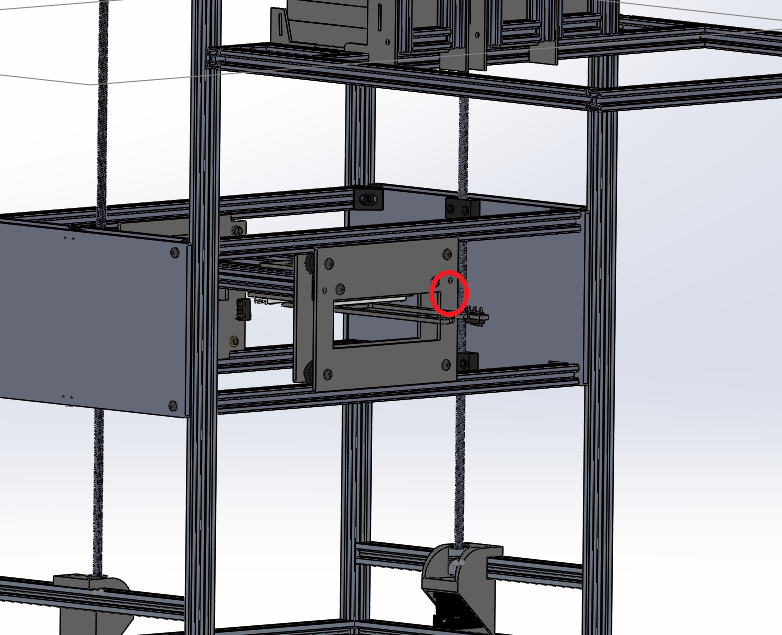
\includegraphics[width=6cm]{images/layerDetectionPosition.png}
					\caption{Image of where a linear hall effect sensor can be placed ({\color{red}\textbf{red}} circle) to detect the layers of the platform, if small magnets are placed at each layer.}
					\label{fig::layerDetectionPosition}
				\end{wrapfigure}
	
		
		The dish containers worked generally fine, but had some issues which must be addressed. The structures are stable and can easily hold a stack of dishes or plates, while the room for the PCB in the bottom for electronics is nicely hidden and will to some extend protect from potential dripping liquids. During the tests, a 6mm POM sheet could perfectly be hold in place by the grooves in the alu profiles. Potentially a piece of POM can be cut in a CNC machine and the PCB mounted onto the 6mm POM, for easy access to potential electronics in the bottom. To make it even more accessible, the design of the containers are slightly modified to have a 90x20mm 3mm POM to hold the PCB board in place, and the skeleton of alu profiles in the back is lifted by 23mm (see figure \ref{fig::containerSkeletonLiftet}). Now the back of the multiplate containers are only supported be 2 vertically positioned 3mm POM sheets, which can appear rather fragile. But the center and front are supported by 3 alu profiles, that will take the larger amount of the dish container's weight, which protects the rear 3mm sheets from breaking.
		
				
		
		\begin{wrapfigure}{r}{0cm}
			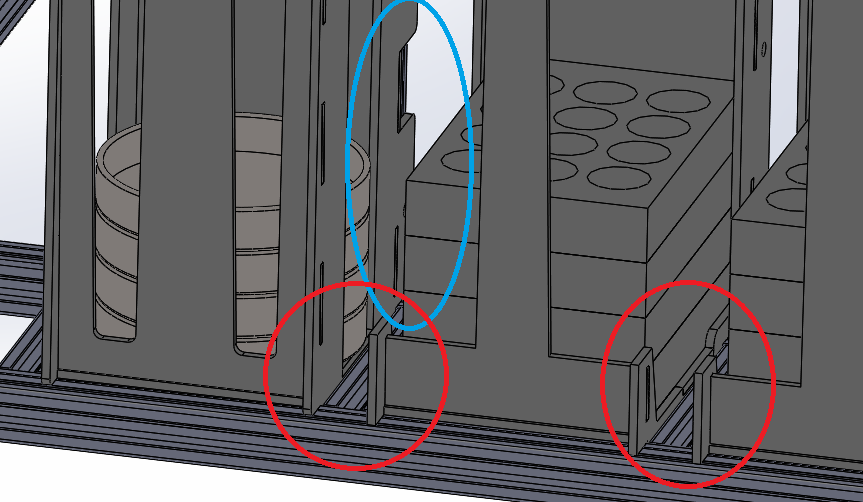
\includegraphics[width=6cm]{images/newContainerDesign.png}
			\caption{Containers where the alu profiles at the side have been moved to the center ({\color{blue}\textbf{blue}} circle) and the containers are only separated by a 20mm alu profile ({\color{red}\textbf{red}} circle). These 20mm should leave enough room for the 10mm wide arm to reach a dish/plate.}
			\label{fig::newContainerDesign}
		\end{wrapfigure}
		
				
		The alu profiles at the sides of the containers are claiming a lot of space and restricting the amount of dish containers there can be placed in the frame for the containers. By moving the alu profiles into the center instead of leaving them on the sides, 40mm can be spared with each container. Naturally there has to be room for the arms of the gripper to get into the dishes/plates without risking to collide with the sides of the containers. The 20mm alu profile, which separates each container and making sure that the user positions them correctly, should give enough room for the arms of the gripper (see figure \ref{fig::newContainerDesign}). This change reduces the width of the containers with 14.3 \%\footnote{Each container was 140mm wide, but is now 100mm wide. Including the 20mm alu profile for separating the containers, the new width is $\frac{100 + 20}{140} = 85.7 \%$ }
		
		
		The top of the Petri dish container had both advantages and disadvantages: As mentioned in \ref{subsub::1iterationLayerDetection}, the top provided a good location for distance sensor to be mounted, but it also gave the use a hard time when filling/emptying the container, as each dish had to be carefully handled if no fluids, etc. were to be spilled. 
		
		This is a big disadvantage, but the fact that the dishes are more protected with the top and they won't all fall out of the container, if it is dropped, seems to be strong enough for trying the idea one more time: The top is now raised with 10mm, which give the user a total of 40mm when inserting/removing dishes.\\
		
		Thoughts about adding magnets to the front and thereby provide a snap-on solution to remove the entire front was also considered. These magnets could interfere with the hall sensors (if those are to be used), but also increased the hassle of producing the container quite a lot, as they most likely would be glued on and should have counterparts of metal, which also should be mounted. It seems to increase the production too much, so the idea is not abandoned yet, but the raising the top 10mm is first tried out.
		
		
		
		When it comes to the front of the plate container, the more open front, compared to the dish container, didn't provide enough support for the plates during transportation by the user: The plates didn't fall out of the container, but was not held properly in place. Therefore the design will change to remind more of the dish container and provide support for the plates in all four corners.
		\begin{wrapfigure}{r}{0cm}
			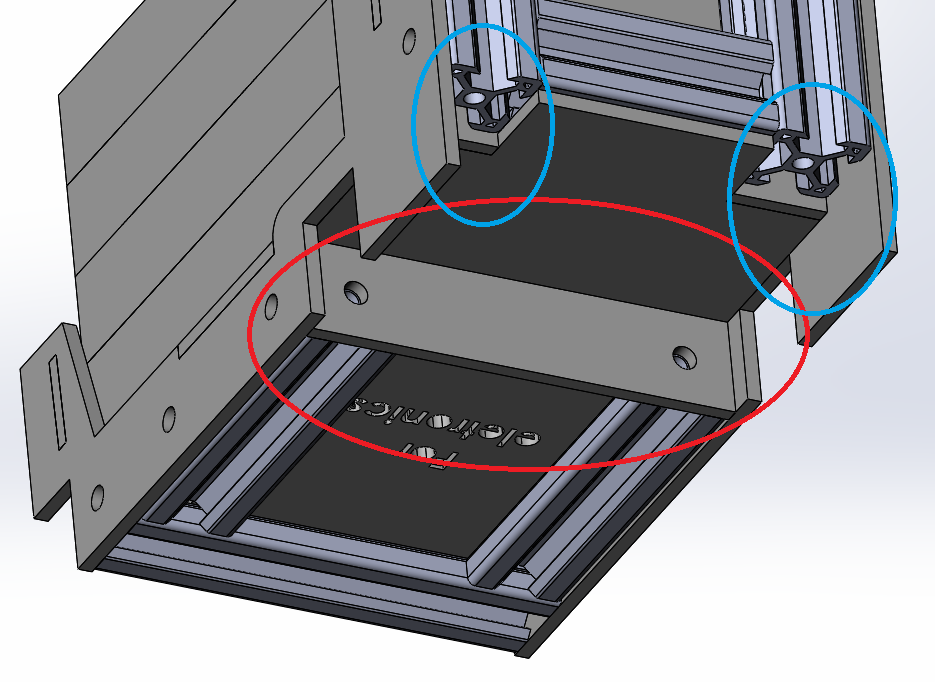
\includegraphics[width=6cm]{images/containerSkeletonLiftet.png}
			\caption{Containers where the rear alu profiles are lifted 23mm ({\color{blue}\textbf{blue}} circle) and 90x20mm 3mm POM sheet to hold the PCB board in place ({\color{red}\textbf{red}} circle).}
			\label{fig::containerSkeletonLiftet}
		\end{wrapfigure}
		
		\subsubsection{Misc. design decisions}
		\begin{wrapfigure}{r}{0cm}
			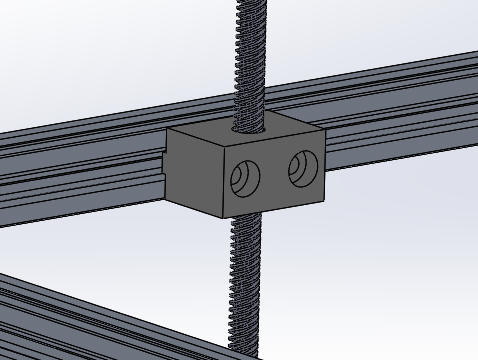
\includegraphics[width=6cm]{images/leadScrewSupport.png}
			\caption{Small plastic piece to prevent collisions with the frame, when the module is in a lower position.}
			\label{fig::leadScrewSupport}
		\end{wrapfigure}
		
		One of the first experiences with the module is that the moving part is too heavy to hold to itself in a lifted position. Because of too steep an angle of the lead screws, the moving parts will sometimes start to move down, when no power is added to the stepper motors. The best solution would be to use a geared stepper motor and possibly a bigger stepper motor (NEMA 17), but lacking geared stepper motors, this project will try with just a NEMA17 motor.
		
		As the module will move to a lower position, when no power is added, the endstops in the vertical direction will be damaged as these currently are the only support for the module in the lowest position. Therefore the endstops have been moved a bit, so the end of the endstop is completely aligned with the end plate it is mounted to. In this way the endstops can still be activated, but not risking stress under the weight of the moving parts.
		
		Another problem with the lead screws is, that they are unsupported in the top, which results in collisions with the frame when the module is in a lower position. This is addressed by designing a small piece of plastic (see figure \ref{fig::leadScrewSupport}), that is mounted to the top of the frame, allowing the lead screw to spin freely with a gap of ~1mm.
		
		
				
	\subsection{2nd iteration}
	
		The 2nd iteration was quite successful, but some unexpected experiences was done about, i.e. the points of contact for the right arm would not be parallel with the edge of a multiplate, when the pressure was added. Other experiences were more successful as, i.e. the hall effect sensor for the layer detection and the US sensor for determining, how many dishes/plates that are in a container.
		
		\subsubsection{Gripping functionality}
		An unfortunate experience was noted during these tests, as the force from the servo made the right arm bend a bit. This resulted in the two points of contact wasn't parallel with the edge of the multiplate, and for that reason the points of contact was limited to only two. This made the plate occasionally lean forward and sometimes collide with either the plate container or the layer of the laboratory platform.
		
	
				
		The best way to address this problem is to make a design for the fingers that is somewhat flexible as, i.e. the one on figure \ref{fig:halfCircle}. But as mentioned in the initial design, this may also lead to misalignments itself if the design is not lose enough: If the half circle has the slightest friction between it and the arm, the half circle may end up pushing the plate out of alignment, when grabbed. As an attempt to address this serious problem, a larger fillet is added where the arm is bend by 90$^{\circ}$ (see figure \ref{fig:gripperLargerFillet}).
			 		
		
		The screws turned upside-down to handle a Petri dish along with the lid, \textit{did} work, when the screws were changed from M3 to M5 screws, because of the larger heads. But as the point of contact then was moved ~20mm down, it introduced a large twisting in both arms. The arms didn't break during the times it was tested, but for more extensive periods, the plastic will most likely start to shape accordingly to the twist or even break. So the original idea of having the screws in the normal position was kept.
		\begin{wrapfigure}{r}{0cm}
			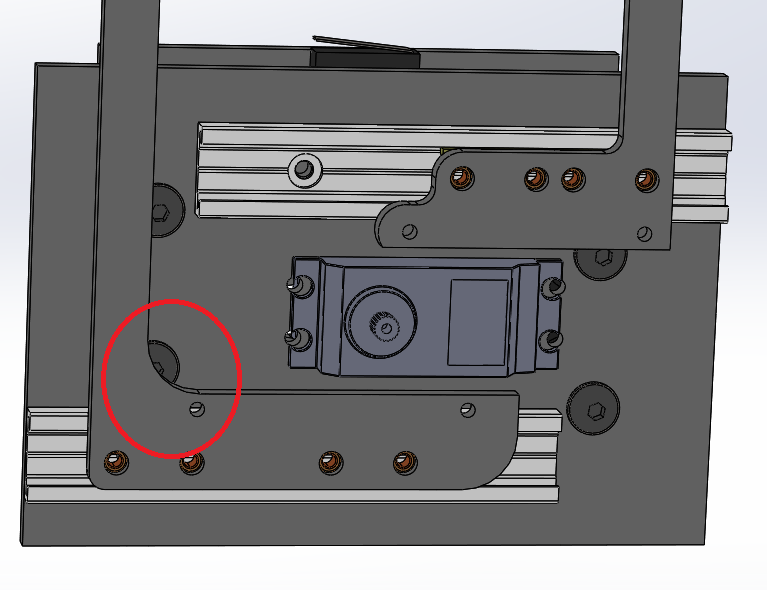
\includegraphics[width=6cm]{images/gripperLargerFillet.png}
			\caption{Gripper from the bottom. The {\color{red}\textbf{red}} circle indicates where the size of the fillet has been increased to prevent the arm from bending under pressure.}
			\label{fig:gripperLargerFillet}
		\end{wrapfigure}
		\begin{wrapfigure}{r}{0cm}
							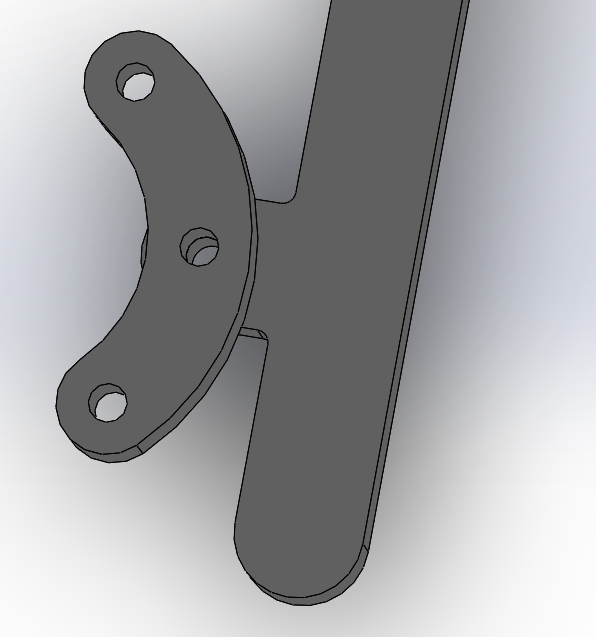
\includegraphics[width=6cm]{images/halfCircle.png}
							\caption{The "half circle" idea, where the two fingers now can adjust to, i.e. the sides of a multieplate to get a better grib.}
							\label{fig:halfCircle}
						\end{wrapfigure}
		The increased distance between the fingers on the right arms, gave a better and more firm grip, when manipulating either a dish or a plate. An even bigger distance between the finger would give an even better grip, but the dish container is preventing this as grooves in the sides can't be increased in size. \textit{If} they were to be increased in size, the dishes would be able to slide more during transportation and the self-aligning idea of the leaning grooves would be worsened.
		
		
		\subsubsection{Layer detection}
		
		The hall effect sensor placed on the moving parts of the module (see figure \ref{fig::layerDetectionPosition}) was first placed on the inside, to hide it for ethical reasons. This \textit{did}work, but determining the location of the layers was not precise enough. After moving the sensor to the outside and bring it ~4 mm closer to approximately 15 mm from the magnets, the determining was a lot better.
		
				
		\subsubsection{Dish containers}	
		
										
		The US sensors mounted in the top of the containers (see figure \ref{fig:dishContainerUsSensor}) are reliably measuring the distance to the top dish/plate - especially as the distance between the top of the container and the top part of the sides (which also is the top of the dishes/plates) are 40 mm and the US sensors works reliably down to 30 mm. A micro controller in the bottom of each container is not needed, as the measuring can be conducted by the same controller, which takes care of the motions, etc.

		The fact that the top is still there can be a bit annoying, when removing/adding dishes to the container, even though it has been increased by 10 mm. The top can't be completely removed from the design, now that it works as a mounting position for the US sensor, but to ease the usability, a cut can be inserted between the lower part of the container and the top. This will allow the user to slide up the top, when accessing the dishes and lower it again when done - unless gravity can ensure that the top always will drop down. This idea will increase the possible distance between the top and the top of the sides from 40 mm to 85 mm.\\
		
		By changing the front design of the plate container to support the plates in all four corners, the plates are now kept better in place. The plates are able to move a total of 4 mm to the sides, which may lead to the plates not being positioned correctly into the container, when inserted by the dispenser module. During the hand controlled tests, this didn't happen, but further tests should be conducted, when the module are performing these movements itself.
		
		\begin{wrapfigure}{r}{0cm}
					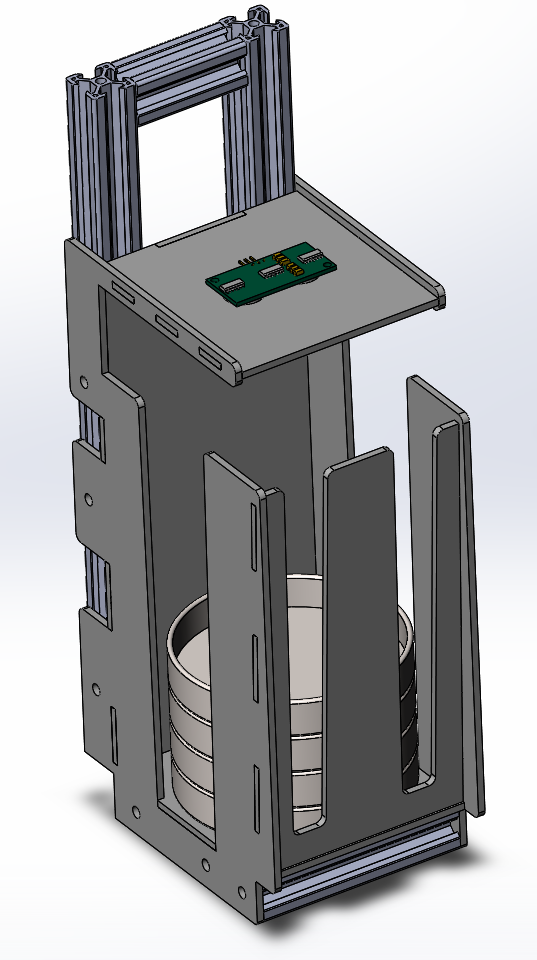
\includegraphics[width=6cm]{images/dishContainerUsSensor.png}
					\caption{Dish container where the Parallax ultrasound sensor is mounted on the top.}
					\label{fig:dishContainerUsSensor}
				\end{wrapfigure}
		\subsubsection{Misc. design decisions}
		The lack of geared NEMA motors, which resulted in an increase of motor size, turned out to make the moving parts a bit more reluctant to move down, when the power is shut off. This isn't nearly enough to be considered as a reliable solution, so the geared solution or, i.e. solenoids to prevent the motors from turning when not powered, is the correct way forward.\\
		
		The support for the lead screws to prevent them from colliding with the frame worked well. There is a slightly risk that they may be worn down, but given the fact that there is no pressure between the supports and the lead screws, the wearing down is estimated to be within years of constant use.
			
			
	\subsection{Final result}
		The dispenser module (see appendix \ref{app:finalResult} for final result) is now starting to look more toward and actual usable product, even though there still are a few issues, which must be addressed first. One of the things is that throughout the design process, the tests have been conducted by simply moving the parts by hand. Even thought it shouldn't differ much, the true picture of the design is first revealed when the module is running by itself.
		
		The absolute main part of the firmware has been developed, where it is running on a Teensy 3.2 and controlling/reading the motors and sensors through the custom designed PCB (see figure \ref{fig:pcb}). The sensors in the module, i.e. the endstops, are in general connected so that a constant power flowing into the pin of the controller, while also having a pull-down resister in the circuit. This set up will save 1 wire to each of the sensors\footnote{10 in total, when allowing for up to 4 dish/plate containers. 6 of the 10 is for endstops.} with this set up. The reason for not letting the constant signal to be ground, is that a potential damage to the signal wire, would not be discovered.
		
			
		\subsubsection{Gripping functionality}
		The gripper is currently able to handle Petri dishes, but increased size of the fillet at the right arm, didn't help much towards not losing the grip when handling multiplates. The gripper is moving in a smooth and firm way, though, and has a very compact design.
		
		With the increased distance between the fingers on the right arm, the gripper can handle a Petri dish that is up till 15 mm off its intended position. A multiplate with a with of 86 mm may be up till 7 mm off.
		
		
		\subsubsection{Layer detection}
		The layer detection is working very well with the linear hall effect sensor mounted on the outside of the POM. The determination of the layers position can be done within ~4 mm, when no metal or other magnetic interferences are nearby the magnet.
				
		\subsubsection{Dish containers}	
		The dish containers for both the Petri dishes and the multiplates are holding the dishes/plates firmly in the correct position. They have also been designed to align the dishes/plates in case the gripper is inserting them into the container un-centered.
		
		The containers have a top to protect the dishes/plates, but also for holding the US distance sensors, which is working well for detecting the height of the dishes/plates. During the test, it was experiences that the top limited the user from adding/removing dishes or plates to the container, which has been addressed by allowing the user to slide up the top and provide a gap of 85 mm - gravity will often, but not always, make sure the top is dropped down to its correct position to give an accurate height of stack inside.
		
		The firmware has been designed to automatically detect when a container is inserted/removed by adding a small resistor to PCB in the bottom of the container. The container can hold a PCB at 76-81x60 mm, depending on the container type, which easily can be inserted be loosing two screws and remove a small piece of POM (see figure \ref{fig::containerSkeletonLiftet}).
		
		\subsubsection{Misc. design decisions}
		
		Initially the lead screws were  colliding with the rest of the module, when the moving parts where in a lower position. This was solved by designing and 3D print two brackets, that allow the lead screws to be in the intended position $\pm$ 1 mm. The angle of the thread in the lead screws were too steep, which meant that the weight of the moving parts would force the stepper motors to start spinning when no power was added, slowly lowering the moving parts. This problem hasn't been addressed, but a less step lead screw or adding a gear to the stepper, should do the work.
			
		The frame to be placed in top of the laboratory platform, for holding the containers, is able to force the user to not place the containers in wrong positions. It is supporting the containers in two locations and is mechanically connected to the rest of the module by just two corner brackets
			
	\section{Software}
		\subsection{Choice of controller}
		One of the first decisions, when it comes to writing firmware for robot, is what architecture it shall run on. In this project it is obvious to use a micro controller, that is more or less related to the Arduino family\footnote{Overview of the Arduino family: \url{https://www.arduino.cc/en/Main/Products}}, as the RepRap community\footnote{RepRap community: \url{http://www.reprap.org/}} has developed several successful 3D printers based on the Arduino Mega board. The mechanical design of the dispenser in this project, can be compared to a standard 3D printer, as both are based on 3 axis, controller by stepper motors and endstops. The dispenser module has connectors to detect, when a stack of plates are inserted or removed, as well as initial measuring for amount of current going to the servo in the gripper - but all of these are basic electrical circuits that can be handled by most controllers.
		
		The choice was between the Arduino Mega or the Teensy 3.2, LC (Low-Cost) or 2++. All are based on the Arduino language and is roughly the same in terms of number of pins, but the Teensys are designed on ARM processors, which implies the execution of code to be a lot faster (between 3-12 times faster, depending on the model). Both the Arduino Mega and the Teensys are open-source and can be designed into a custom made PCB\footnote{PCB is short for Printed Circuit Board.} to keep the future aspects in mind. The price of the Teensy is between half and one third of the Arduino Mega and the Teensys have a better variety of types of IO-ports.
		
		The choice of board ended with Teensy 3.2 and Teensy LC, which resulted in created an electrical setup (see figure \ref{fig:pcb}). If the Arduino Mega was used, it could have been beneficial to use the RAMPS 1.4.2\footnote{Blueprints of the RAMPS 1.4.2: \url{https://github.com/GermanRepRap/Ramps-1.4.2}} shield, which is designed by the RepRap community.
		
		One of the key points of choosing the Teensys was to make sure that the controller could execute the code fast enough to ensure a responsive API to the firmware, while allowing the module to execute queued commands at the same time: The stepper motors must be triggered at the correct time to ensure a proper motion control. 
	
	
		\subsection{Firmware}
		As written in the \ref{subsec_Goals} one of the important parts of this project is to have responsive API to the firmware. This means that any commands and responses must be handled while executing smooth motions. This is achieved in two steps:
	
		\begin{table} %{l}{8cm}
			\begin{center}
				\begin{tabular}{|| c | p{5cm} ||} 
				\hline
				Command & Description\\ [0.5ex] 
				\hline\hline
				d\textless stack number\textgreater & dispense a dish/plate from stack \textless stack number\textgreater . \\ 
				\hline
				r\textless stack number\textgreater & remove dish/plate form platform and put it in stack \textless stack number\textgreater .\\
				\hline
				c & calibrate. This will automatically determine the available dimensions and any layer positions.\\
				\hline
				o & move to origo. \\
				\hline
				g\textless x\textgreater,\textless y\textgreater,\textless z\textgreater,\textless a\textgreater & go to step position (\textless x\textgreater,\textless y\textgreater,\textless z\textgreater) and open (\textless a\textgreater \space is 0) / close (\textless a\textgreater \space is 1) arms \\
				\hline
				i\textless x\textgreater,\textless y\textgreater,\textless z\textgreater & define insertion / removal point at step position (\textless x\textgreater,\textless y\textgreater,\textless z\textgreater).\\
					 \hline
				l & get layer positions in mm. \\
				\hline
				w & get total available width in mm. \\
				\hline
				h & get total available height in mm. \\
				\hline
				p & get current position in mm - format: (\textless width\textgreater ,\textless height\textgreater ) \\
				\hline
				s & get amount of dishes in stacks - format: Int array width dish amount for each stack. -1 if no stack in place\\ %[1ex] 
				\hline
					\end{tabular}
			\end{center}
			\caption{Available commands and descriptions. Each command must be separated with a semicolon.} \label{table:commands}
		\end{table}	
			
		\begin{enumerate}
		\item The UART buffer is big enough to hold incoming characters for a little while, so by keeping the commands simple and by reading a single character every time the loop\footnote{The loop is the method in the code, which will be run again and again. The two main methods in Arduino is the setup(), which is run once and then the loop().} is executed, it will constantly empty the buffer and any requests for data can rapidly be returned. Normally, this would be implemented with interrupts, but to prevent wrong timings for triggering the stepper motors, when receiving a large amount of commands at one time, this has been avoided.
		\item The AccelStepper library\cite{accelStepperLibrary_webpage} will trigger the stepper motors at the correct times, to handle acceleration, deceleration and steady motions with as good as no time off-sets. The AccelStepper is also called once in every execution of the loop and if a new step is ready to be triggered, it will.
		\end{enumerate} 
		
		Another subject that has been taken into account during the writing of the firmware, is the fact that it is running on a micro controller. This means that only a sparse amount of memory is available. Therefore the code has two simple data structures. The first is symbolizing a command from table \ref{table:commands}, which only consists of an enum and four variables. 
		
		When data is received from the UART and translated into a valid command, it will be stored in a queue, until all previous commands has been executed. When the command is ready to be executed, it will be translated into a series of motions - which are stored in another queue. By doing this, the minimum amount of space is used and the risk of runtime errors are minimized. Once a valid command is received an acknowledging \textit{OK} is replied - in case of an invalid command, the host system will receive information about this, too. The default limit of commands in the command queue is set to 64 and the motion queue has a limit of 32.
		
		In the time of writing only the endstops has been implemented with interrupts. Later the detection of changed in containers being added/removed should be implemented in the same way.
		
		
	
	
	\section{Discussion}
		The final result of the dispenser module is able to perform primary requirements, which can be expected from such. During the project, there was experienced some severe delivery issues of the hardware, as it wasn't delivered until less than 1 month before the deadline. Even though the firmware was written during the waiting time and all possible tasks was prepared for the receiving of the hardware, the nearby deadline, forced prioritizing the main part of the project: The design. The nearly done firmware was therefore abandoned and only short tests, single-action pieces of code and movements by hand were used to evaluated over the mechanical design.
		
		These kind of things \textit{will} happen sometimes, but one thing that can learned from this, is to always have lots of supplies - even before the project begins. The best approach is to take the risks (in this case the supplier) out of the equation and have plenty of all potential needed parts - no-matter what the financial department might say...\\
		
		\begin{wrapfigure}{r}{0cm}
			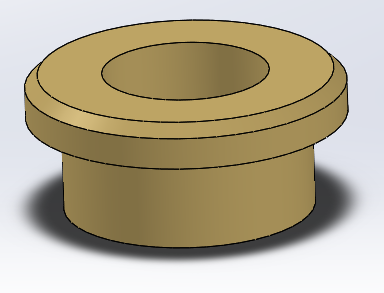
\includegraphics[width=4cm]{images/microbarb.png}
			\caption{Microbarb is small piece of brass, which can be hammered into a hole of, i.e. POM. The microbarb is provided with metric threading at the inside and can be used as a replacement of a nut.}
			\label{fig::microbarb}
		\end{wrapfigure}
		
		All of the parts are standard parts, which can be acquired in most places. Nearly all of the parts are even open-source, as only the microbarbs (see figure \ref{fig::microbarb}) and the Parallax distance sensor isn't. The microbarbs might even be needless in some parts of the design by threading the holes in the POM to fit the screws.
		
		The approach about using standardized and mainly open-source hardware is to allow users of this dispenser to, first of all be able to get the parts easily and at a low cost, but also to be able to produce the spare parts himself, if something breaks. Compared to an industrial dispenser, this removes the waiting time and the high price for having a technician to come and repairing it. The fact that the user is able to repair the module by himself, is also one of the design goals for the dispenser (see \ref{subsec_Goals})!
		
		Given the use of standard hardware and especially specific design decisions, the module is also created to fit the majority of current available laboratoty platforms: The module is placed next to the platform and the frame for the dish/plate containers are placed on top of the platform. The weight of the frame for the containers and the containers are mainly made of lightweight materials in terms of aluminium and plastic. It is therefore highly unlikely that the platform should \textit{not} be able to carry the weight of these! Most loboratoty platforms are also shaped as cubes, which makes it easy to fit the design module.
		
		The frame for the containers are put together with the rest of the module by 2 corner brackets, which is all there is needed for setting up the dispenser module physically. The part of the module, that is placed next to the platform, is not heavy, but weights enough to eliminate any doubts about the module not staying in place. There is even added small rubber feet, so that the module can not only be adjusted, but minor vibrations, will not slowly move the module.\\
		
		The Petri dish and multiplate containers are able to hold the dishes/plates firmly in place - not just during use of the module, but also when a user is transporting the containers from a to b. The type of dishes/plates that are placed into the container frame, is detected at runtime by measuring the voltage across a resister (if any) in the bottom of the container, while the Parallax sensor in the top of the container provides the height of the stack of dishes/plates. The resister in the bottom is a simple and extremely low-cost solution to detection the dish/plate type, while the distance sensor costs ~30 USD. The cost of the distance sensor might be lowered by testing other sensors, that also has both an emitter and receiver for the US waves, as this is what separated the sensor from the other ones tested.
		
		
				
		The size of the multiplates appear to be the same, no-matter how many wells, they contain. The Petri dishes come in different sizes, but the dish container (and the plate container, too) can be resized to fit the wanted size of dishes/plates. The only requirement is that they keep the design of the bottom, so that they will fit into the frame for the containers (see figure \ref{fig::containerFitFrame}). \\
		
		
		Even though the containers are able to handle different types and sizes of dishes and plates, one of the later iterations showed that the gripper is not matured enough to have a firm grip on a multiplate: When the pressure from the servo increased, the arms would bend slightly, having the right arm with two fingers not be parallel with the plate. This resulted in only two points of contact, which is not enough for a good grip. Ideas about using a half circle (see figure \ref{fig:halfCircle}) to hold the two fingers instead of the current rigid design, was considered. These ideas was already from the initial design abandoned as they could lead to misalignments, if there was the just the smallest amount of friction between the arm and the half circle.\\
		
		\begin{wrapfigure}{l}{0cm}
			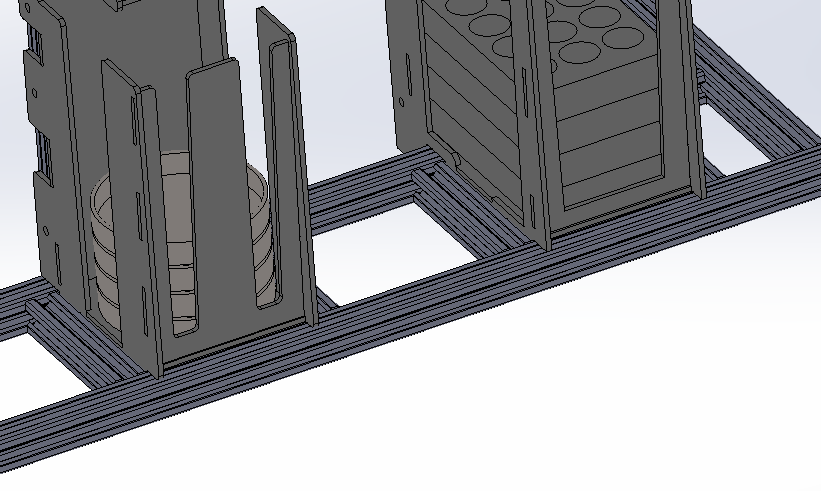
\includegraphics[width=6cm]{images/containerFitFrame.png}
			\caption{When resizing the container, the only requirement is that the dimensions of the bottoms is left intact, so it will fit into the frame for the containers.}
			\label{fig::containerFitFrame}
		\end{wrapfigure}
		
		One of the design goals is also that the dispenser module can detect any layers, there might be in the laboratory platform. As described in \ref{subsec:intialDesign}, most platforms consists of three layers: One for analising, one for manipulating the dishes/plates and one for tools. By determinate the positions of the layers, the dispenser module can easily be set up to use one of these layers as insertion/removal point for clean/used dishes and plates. By testing 8 different sensors\footnote{The 8 different sensors were 3 ultrasound, 2 IR, 1 level swicth and 2 hall effect sensors.}, it was concluded that the best way to detect the layers, is by attaching a small magnet to each layer\footnote{Note the direction of the magnet, when attaching it to the layer. The direction \textit{will} matter to the hall effect sensors.}, the linear hall effect sensor can then provide information about the layer's position.
		
		Initially the idea was to combine the device for detecting the layers with the one detecting the height of the dish/plate stack in the containers. As it turned out, the only feasible way was to separate these two functions, as the technical aspect and the size of the sensor couldn't be combined to fit at the tip of the grippers arm and reliably detect objects close by. 
		
		The hall effect sensor is mounted in the outside of the moving parts of the module (see figure \ref{fig::layerDetectionPosition}), the sensor will return larger values the closer it is to the magnet. Simple use of math can determine the position of the layer - tests shows, that the precision is less than 4mm.\\
		
		Even thought the firmware isn't completely finished, it \textit{is} written in a way that addressed the design goal about Responsive Control. The firmware is able to alternate between reading incoming data and taking care of the motor controls. This is done by simply reading a single char at a time, while leaving the rest in the buffer until the next time. Same goes for the motor controls, which also can take care of accelerating, decelerating or keeping a steady speed.
		
		The firmware is written so that it respects the small amount of space in a micro controller, as any valid incoming command is stored. It is not until the very last moment the command is translated into a sequence of motions, which keeps the used space to a minimum.\\
		
	\newpage
		To summarize which of the design goals, that has been achieved in this project, they have been listed below (refer to \ref{subsec_Goals} for descriptions of the goals):
		\begin{itemize}
			\item \textbf{Modularity} The dispenser module is simply placed next to the laboratory platform.
			\item \textbf{Versatility} The containers can support both Petri dishes and plates, but the gripper is not matured enough to handle the plates.
			\item \textbf{Usability} Dish/plate containers can be added/removed at runtime, which will be detected by the module.
			\item \textbf{Flexibility} The module can be placed next to the laboratory platform and the dish/plate containers on top of the platform, as most platforms are shaped like a cube.
			\item \textbf{Increased feedback} The dispenser automatically detect any layers of the platform by detecting positioned magnets.
			\item \textbf{Repairability} Spare parts for the module can easily be made or bought at a very low cost.
			\item \textbf{Responsive Control} Controller can handle incoming/outgoing data while controlling the motions of the dispenser.
		\end{itemize}
	
				

		
	\section{Conclusion}
	Even thought the project suffered from severe delivery problems of the hardware, as this just arrived less than 1 month before the deadline, and the delayed the entire project, the project is still successful.
	
	By using almost nothing than open-source, but all standardized hardware, the construction of the designed dispenser module can be created in most places. This makes it possible for most people to benefit from this project, but also addresses one of the design goals about the user easily being able to repair the module in case it gets worn down or breaks.
	
	The design goals was created to have something realistic to aim for throughout the project. In the current state, the dispenser module fulfils 5 out of the 7 design goals. Those lacking are the Versatility and the Responsive Control. The Versatility is not fulfilled as one of the later iterations reveals that the arms will bend under the pressure from the servo and for that reason not have a good grip of the multipates. The handling of the Petri dishes is very good, though - just like the containers for the dishes and plates works very well. The design of the containers also allows the controller to measure the height of the stack and detect which kind of dish/plates it is holding - defined by a small resister in the bottom.
	
	The Responsive Control \textit{is} actually fulfilled, as the firmware is written with respect to not only incoming/outgoing data, but also the controls of the motions. The firmware will always be able to respond to incoming request, no-matter which state it is in. But since the firmware also was delayed from the delivery issues, the firmware is only nearly done, and one can therefore not guarantee that issues, which affects the responsive control might occur - even though this is \textit{highly} unlikely!
	
	As the focus of this project is on the mechanical design, the further development and maturing was done by small pieces of codes to simulate the actions related to the parts being matured. Therefore tests throughout the project was done and reflected upon, even if it left out post and pre motions/actions, which in most cases wouldn't affect the test anyway. This should be done later on, just to be absolutely sure, though.
	
	All of the 5 other design goals are implemented as the dispenser can detect layers of the laboratory platform it is connected to, easy to setup, fits the majority of platforms, etc.
		
	
	
	
	\section{Acknowledgements}
	The author would like to thank primarily Kasper Støy and Andrés Faina from the IT University of Copenhagen for supervising this project, but also REAL Lab, PIT Lab and IxD Lab for providing temporarily sensors, misc. equipment and especially space for building the project.
	
	
	\newpage
	\bibliographystyle{plain}
	\bibliography{references}
	\newpage
	
	\appendix
	\section{Final result}\label{app:finalResult}
	\begin{wrapfigure}{r}{0cm}
		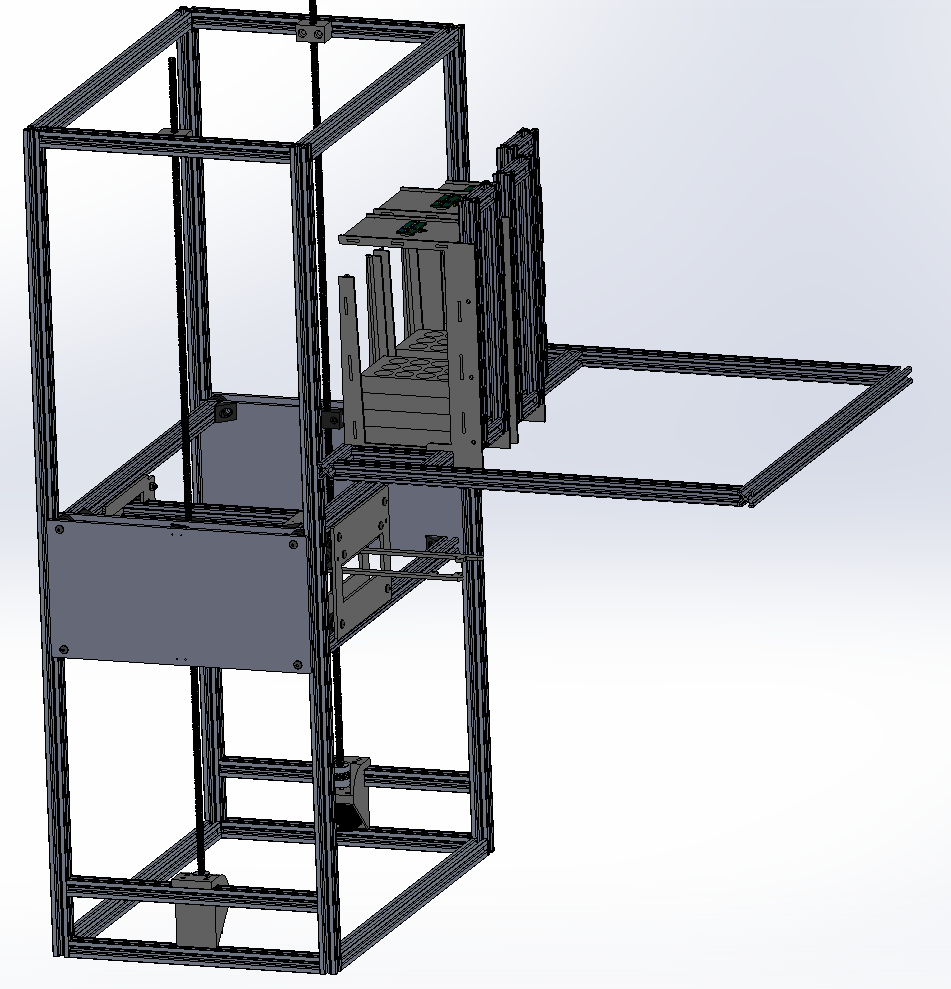
\includegraphics[width=15cm]{images/completeModule.png}
	\end{wrapfigure}
		
\end{document}






